\documentclass{ltxdockit}
\usepackage{btxdockit}

\usepackage[T1]{fontenc}	
\usepackage[utf8]{inputenc}		
\usepackage[english]{babel}

\usepackage[bitstream-charter]{mathdesign}
%\usepackage{hyperref}

\usepackage{booktabs}
\usepackage{microtype}

\lstset{
    basicstyle=\ttfamily,
    keepspaces=true,
    upquote=true,
    frame=single,
    breaklines=true,
    postbreak=\raisebox{0ex}[0ex][0ex]{\ensuremath{\color{red}\hookrightarrow\space}}
}

\KOMAoptions{numbers=noenddot}
\addtokomafont{title}{\sffamily}
\addtokomafont{paragraph}{\spotcolor}
\addtokomafont{section}{\spotcolor}
\addtokomafont{subsection}{\spotcolor}
\addtokomafont{subsubsection}{\spotcolor}
\addtokomafont{descriptionlabel}{\spotcolor}
\setkomafont{caption}{\bfseries\sffamily\spotcolor}
\setkomafont{captionlabel}{\bfseries\sffamily\spotcolor}

\makeatletter
\patchcmd{\paragraph}
  {3.25ex \@plus1ex \@minus.2ex}{-3.25ex\@plus -1ex \@minus -.2ex}{}{}
\patchcmd{\paragraph}{-1em}{1.5ex \@plus .2ex}{}{}
\makeatother

\hypersetup{%
  pdftitle={The tikzducks package},
  pdfsubject={using ducks in tikz},
  pdfauthor={samcarter},
  pdfkeywords={tex, latex, tikz, ducks}
}

\usepackage{tikzducks}
\usepackage{xspace}

\newcommand{\tikzducks}{\texttt{tikzducks}\xspace}

\title{The \tikzducks Package}
\subtitle{using ducks in tikz}

\begin{document}

\begin{center}
	{\LARGE \textbf{The \texttt{tikzducks} Package (version 0.1)}}
	
	\large using ducks in \texttt{tikz}
	
	samcarter (alias 
	
\begin{tikzpicture}[scale=0.3,baseline=5pt]
		\duck[body=yellow!50!brown!50!white, 
					longhair=red!50!brown, 
					jacket=blue!50!black]
	\end{tikzpicture}%
	)
	
	\url{https://github.com/samcarter8/tikzducks}

	\today
\end{center}

\section{Introduction}
\label{intro}

The \tikzducks package is a latex package for ducks to be used in \texttt{tikz} pictures. This project is a continuation of an answer at TeX.Stackexchange (\url{https://tex.stackexchange.com/a/347458/36296}).

This package is work in progress (and will probably never be really finished as there is an infinite amount of things which could be added), therefore I would be happy to hear your feedback and ideas how to improve the package. The source code can be found on \url{https://github.com/samcarter8/tikzducks}, including a bug tracker, please make constructive use of it!

\subsection{License}

Copyright \textcopyright\ \texttt{samcarter}. Permission is granted to copy, distribute and\slash or modify this software under the terms of the LaTeX project public licence, version 1.3c \url{http://www.latex-project.org/lppl.txt}

The shown example ducks are purely fictional characters, any resemblance to real persons is purely coincidental and no copyright infringement is intended.

\subsection{Acknowledgements}

I would like to thank a few fellow user from \href{https://tex.stackexchange.com/}{TeX.Stackexchange}: \href{https://tex.stackexchange.com/users/101651/carlatex}{CarLaTeX} for pointing out the overwhelming need of having a \tikzducks package,
\href{https://tex.stackexchange.com/users/3094/paulo-cereda}{Paulo Cereda} for his contagious enthusiasm for ducks (\emph{Quack!}),
\href{https://tex.stackexchange.com/users/4427/egreg}{egreg} for his help to implement the \texttt{\tikzset{}} interface which makes it much easier to adjust the properties of the ducks to fit the user needs and last but not least \href{https://tex.stackexchange.com/users/5763/martin-schr%c3%b6der}{Martin Schr\"oder} for his feedback to the code review

\bigskip\noindent
Without them, this package would not exist!

\section{Usage}

The basic usage is fairly simple, to draw a duck:


\begin{tikzpicture}
\duck
\end{tikzpicture}

To customise this basic duck, the package uses \texttt{pgf} keys. For example to change the colour of the duck:

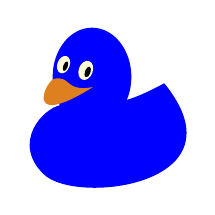
\begin{tikzpicture}
\duck[body=blue]
\end{tikzpicture}

scaling:

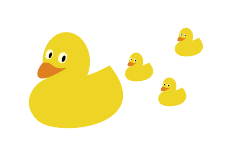
\begin{tikzpicture}[scale=0.6]
	\duck
	\begin{scope}[xshift=90pt, scale=.3, yshift=150pt]
		\duck
	\end{scope}
	\begin{scope}[xshift=60pt, scale=.3, yshift=100pt]
		\duck
	\end{scope}
	\begin{scope}[xshift=80pt, scale=.3, yshift=50pt]
		\duck
	\end{scope}		
\end{tikzpicture}
 
\subsection{Body parts}

The various parts of the duck body can also be coloured independently:

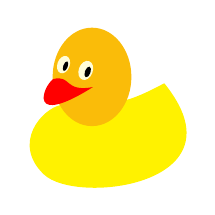
\begin{tikzpicture}
\duck[body=yellow,
			head=yellow!50!orange, 
			bill=red]
\end{tikzpicture}

using the keyword \texttt{grumpy} the shape of the bill can be changed


\begin{tikzpicture}
\duck[grumpy]
\end{tikzpicture}

\subsection{Hair styles}

Some duck also like to have nice hair cuts, several different hair styles are available:


\begin{tikzpicture}
\duck[longhair]
\end{tikzpicture}

\begin{tikzpicture}
\duck[shorthair]
\end{tikzpicture}

\begin{tikzpicture}
\duck[crazyhair]
\end{tikzpicture}

\begin{tikzpicture}
\duck[recedinghair]
\end{tikzpicture}

and of course the colour of each of the hair styles can be adjusted


\begin{tikzpicture}
\duck[longhair=teal]
\end{tikzpicture}

Eyebrows are also part of the package


\begin{tikzpicture}
\duck[eyebrow]
\end{tikzpicture}
\qquad
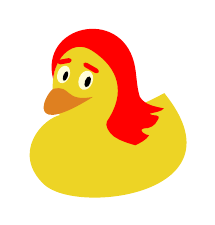
\begin{tikzpicture}
\duck[longhair=red, eyebrow]
\end{tikzpicture}
\qquad
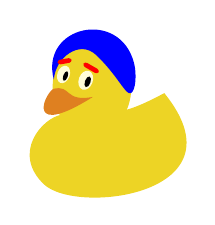
\begin{tikzpicture}
\duck[shorthair=blue, eyebrow=red]
\end{tikzpicture}

\subsection{Accessoire}

There is a multitude of things a duck might need:

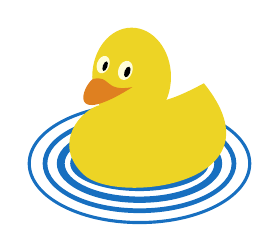
\begin{tikzpicture}
\duck[water=cyan!50!blue]
\end{tikzpicture}
\qquad
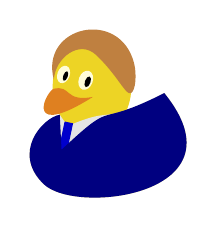
\begin{tikzpicture}
\duck[tshirt=white!80!gray, 
			jacket=blue!50!black, 
			tie=blue!80!black, 
			shorthair]
\end{tikzpicture}
\qquad
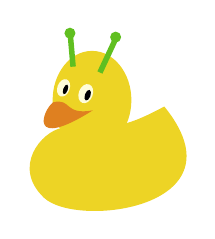
\begin{tikzpicture}
\duck[alien=green!50!brown]
\end{tikzpicture}


\begin{tikzpicture}
\duck[icecream]
\end{tikzpicture}
\qquad

\begin{tikzpicture}
\duck[icecream=brown, flavoura=brown, flavourb=white, flavourc=red]
\end{tikzpicture}
\qquad
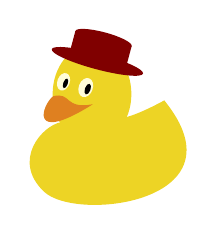
\begin{tikzpicture}
\duck[hat=red!50!black]
\end{tikzpicture}

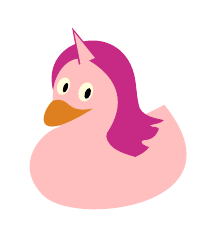
\begin{tikzpicture}
\duck[body=pink,
			unicorn=magenta!60!violet,
			longhair=magenta!60!violet]
\end{tikzpicture}
\qquad
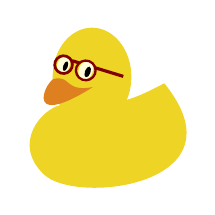
\begin{tikzpicture}
\duck[glasses=red!50!black]
\end{tikzpicture}
\qquad

\begin{tikzpicture}
\duck[sunglasses]
\end{tikzpicture}

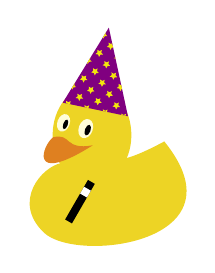
\begin{tikzpicture}
	\duck[magichat,
				magicwand]
\end{tikzpicture}

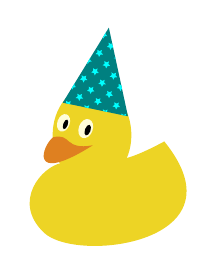
\begin{tikzpicture}
	\duck[magichat=teal,
				magicstars=cyan]
\end{tikzpicture}


\begin{tikzpicture}
	\duck[book=\scalebox{0.5}{\TeX},
]
\end{tikzpicture}


\begin{tikzpicture}
	\duck[book=\scalebox{0.5}{\TeX},
				bookcolour=blue!50!black
]
\end{tikzpicture}

\section{Examples}

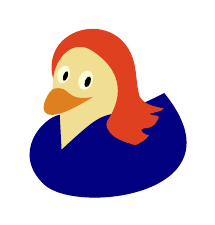
\begin{tikzpicture}
	\duck[body=yellow!50!brown!50!white, 
				longhair=red!50!brown, 
				jacket=blue!50!black]
\end{tikzpicture}
\qquad

\begin{tikzpicture}
	\definecolor{brazilgreen}{RGB}{0,155,58}
	\definecolor{brazilyellow}{RGB}{254,223,0}
	\definecolor{brazilblue}{RGB}{0,39,118}
	\duck[body=brazilyellow,
				jacket=brazilblue,
				shorthair=brazilgreen]
\end{tikzpicture}
\qquad

\begin{tikzpicture}
	\duck[grumpy,
				body=yellow!50!brown!50!white,
				tshirt=white,
				jacket=black,
				tie=black,
				hat=black,
				sunglasses=black]
\end{tikzpicture}

% prof. van duck

\begin{tikzpicture}
	\duck[body=yellow!50!brown!40!white,
				crazyhair=gray!50!white,
				eyebrow,
				glasses=brown!70!black,
				book=\scalebox{0.2}{$E=mc^2$},
				bookcolour=red!20!brown
]
\end{tikzpicture}
\qquad
% knuth
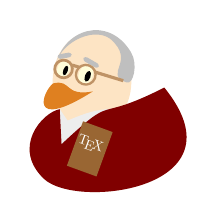
\begin{tikzpicture}
	\duck[body=yellow!50!red!20!white,
				recedinghair=gray!50!white,
				eyebrow,
				tshirt=white!93!black,
				jacket=red!50!black,
				glasses=brown!70!lightgray,
				book=\scalebox{0.5}{\TeX},
				bookcolour=black!20!brown
]
\end{tikzpicture}
\qquad
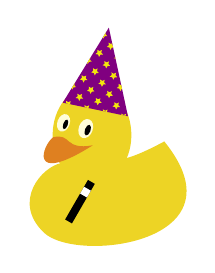
\begin{tikzpicture}
	\duck[magichat,
				magicwand]
\end{tikzpicture}
\qquad



\end{document}

